% Created 2019-06-22 Sat 13:05
% Intended LaTeX compiler: xelatex
\documentclass[12pt,a4paper,oneside,headinclude]{scrartcl}
\usepackage{graphicx}
\usepackage{grffile}
\usepackage{longtable}
\usepackage{wrapfig}
\usepackage{rotating}
\usepackage[normalem]{ulem}
\usepackage{amsmath}
\usepackage{textcomp}
\usepackage{amssymb}
\usepackage{capt-of}
\usepackage{hyperref}
\usepackage{minted}
\PassOptionsToPackage{unicode=true}{hyperref}
\PassOptionsToPackage{hyphens}{url}
\PassOptionsToPackage{dvipsnames,svgnames*,x11names*,table}{xcolor}
\usepackage{lmodern}
\usepackage{amssymb,amsmath}
\usepackage{physics}
\usepackage{ifxetex,ifluatex}
\usepackage{fixltx2e} % provides \textsubscript
\ifnum 0\ifxetex 1\fi\ifluatex 1\fi=0 % if pdftex
\usepackage[T1]{fontenc}
\usepackage[utf8]{inputenc}
\usepackage{textcomp} % provides euro and other symbols
\else % if luatex or xelatex
\usepackage{unicode-math}
\defaultfontfeatures{Ligatures=TeX,Scale=MatchLowercase}
\fi
% use upquote if available, for straight quotes in verbatim environments
\IfFileExists{upquote.sty}{\usepackage{upquote}}{}
% use microtype if available
\IfFileExists{microtype.sty}{%
\usepackage[]{microtype}
\UseMicrotypeSet[protrusion]{basicmath} % disable protrusion for tt fonts
}{}
\IfFileExists{parskip.sty}{%
\usepackage{parskip}
}{% else
\setlength{\parindent}{0pt}
\setlength{\parskip}{6pt plus 2pt minus 1pt}
}
\usepackage{hyperref}
\hypersetup{
pdftitle={Kaggle Fish},
pdfauthor={Rohit Goswami},
pdfborder={0 0 0},
breaklinks=true}
\urlstyle{same}  % don't use monospace font for urls
\usepackage{longtable,booktabs}
% Fix footnotes in tables (requires footnote package)
\IfFileExists{footnote.sty}{\usepackage{footnote}\makesavenoteenv{longtable}}{}
\usepackage{graphicx,grffile}
\makeatletter
\def\maxwidth{\ifdim\Gin@nat@width>\linewidth\linewidth\else\Gin@nat@width\fi}
\def\maxheight{\ifdim\Gin@nat@height>\textheight\textheight\else\Gin@nat@height\fi}
\makeatother
% Scale images if necessary, so that they will not overflow the page
% margins by default, and it is still possible to overwrite the defaults
% using explicit options in \includegraphics[width, height, ...]{}
\setkeys{Gin}{width=\maxwidth,height=\maxheight,keepaspectratio}
\setlength{\emergencystretch}{3em}  % prevent overfull lines
\providecommand{\tightlist}{%
\setlength{\itemsep}{0pt}\setlength{\parskip}{0pt}}
\setcounter{secnumdepth}{0}
% Redefines (sub)paragraphs to behave more like sections
\ifx\paragraph\undefined\else
\let\oldparagraph\paragraph
\renewcommand{\paragraph}[1]{\oldparagraph{#1}\mbox{}}
\fi
\ifx\subparagraph\undefined\else
\let\oldsubparagraph\subparagraph
\renewcommand{\subparagraph}[1]{\oldsubparagraph{#1}\mbox{}}
\fi
% Make use of float-package and set default placement for figures to H
\usepackage{float}
\floatplacement{figure}{H}
\numberwithin{figure}{section}
\numberwithin{equation}{section}
\numberwithin{table}{section}
\makeatletter
\@ifpackageloaded{subfig}{}{\usepackage{subfig}}
\@ifpackageloaded{caption}{}{\usepackage{caption}}
\captionsetup[subfloat]{margin=0.5em}
\AtBeginDocument{%
\renewcommand*\figurename{Figure}
\renewcommand*\tablename{Table}
}
\AtBeginDocument{%
\renewcommand*\listfigurename{List of Figures}
\renewcommand*\listtablename{List of Tables}
}
\@ifpackageloaded{float}{}{\usepackage{float}}
\floatstyle{ruled}
\@ifundefined{c@chapter}{\newfloat{codelisting}{h}{lop}}{\newfloat{codelisting}{h}{lop}[chapter]}
\floatname{codelisting}{Listing}
\makeatother
\usepackage[dvipsnames,svgnames*,x11names*,table]{xcolor}
\definecolor{listing-background}{HTML}{F7F7F7}
\definecolor{listing-rule}{HTML}{B3B2B3}
\definecolor{listing-numbers}{HTML}{B3B2B3}
\definecolor{listing-text-color}{HTML}{000000}
\definecolor{listing-keyword}{HTML}{435489}
\definecolor{listing-identifier}{HTML}{435489}
\definecolor{listing-string}{HTML}{00999A}
\definecolor{listing-comment}{HTML}{8E8E8E}
\definecolor{listing-javadoc-comment}{HTML}{006CA9}
\usepackage{pagecolor}
\usepackage{afterpage}
\setcounter{tocdepth}{3}
\usepackage{setspace}
\setstretch{1.2}
\usepackage{csquotes}
\usepackage[font={small,it}]{caption}
\newcommand{\imglabel}[1]{\textbf{\textit{(#1)}}}
\definecolor{blockquote-border}{RGB}{221,221,221}
\definecolor{blockquote-text}{RGB}{119,119,119}
\usepackage{mdframed}
\newmdenv[rightline=false,bottomline=false,topline=false,linewidth=3pt,linecolor=blockquote-border,skipabove=\parskip]{customblockquote}
\renewenvironment{quote}{\begin{customblockquote}\list{}{\rightmargin=0em\leftmargin=0em}%
\item\relax\color{blockquote-text}\ignorespaces}{\unskip\unskip\endlist\end{customblockquote}}
\definecolor{heading-color}{RGB}{40,40,40}
\addtokomafont{section}{\color{heading-color}}
\usepackage{titling}
\renewcommand{\arraystretch}{1.3} % table spacing
\definecolor{table-row-color}{HTML}{F5F5F5}
\rowcolors{3}{}{table-row-color!100}
% Reset rownum counter so that each table starts with the same row color
\let\oldlongtable\longtable
\let\endoldlongtable\endlongtable
\renewenvironment{longtable}{\oldlongtable} {
\endoldlongtable
\global\rownum=0\relax}
\setlength{\parindent}{0pt}
\setlength{\parskip}{6pt plus 2pt minus 1pt}
\setlength{\emergencystretch}{3em}  % prevent overfull lines
\usepackage{fancyhdr}
\pagestyle{fancy}
\fancyhead{}
\fancyfoot{}
\lhead{Kaggle Fish}
\chead{}
\rhead{\today}
\lfoot{Rohit Goswami}
\cfoot{}
\rfoot{\thepage}
\renewcommand{\headrulewidth}{0.4pt}
\renewcommand{\footrulewidth}{0.4pt}
% When using the classes report, scrreprt, book,
% scrbook or memoir, uncomment the following line.
%\addtokomafont{chapter}{\color{heading-color}}
\usepackage[default]{sourcesanspro}
\usepackage{sourcecodepro}
\usepackage[margin=2.5cm,includehead=true,includefoot=true,centering]{geometry}
\author{Rohit Goswami,\textsc{\scriptsize\ AMIChemE}}
\date{\today}
\title{Kaggle Fish\\\medskip
\large Univ.ai Project}
\hypersetup{
 pdfauthor={Rohit Goswami,\textsc{\scriptsize\ AMIChemE}},
 pdftitle={Kaggle Fish},
 pdfkeywords={},
 pdfsubject={},
 pdfcreator={Emacs 26.2 (Org mode 9.1.9)}, 
 pdflang={English}}
\begin{document}

\usepackage{soul}
\setul{0.5ex}{0.3ex}
\setulcolor{BurntOrange}
\newcommand{rg1}[1]\{\colorbox{BurntOrange}\}\{\textcolor{white}{#1}\}\}
\newcommand{\rg}[1]\{\ul{#1}\}

\begin{titlepage}
\newgeometry{left=6cm}
\definecolor{titlepage-color}{HTML}{06386e}
\newpagecolor{titlepage-color}\afterpage{\restorepagecolor}
\newcommand{\colorRule}[3][black]{\textcolor[HTML]{#1}{\rule{#2}{#3}}}
\begin{flushleft}
\noindent
\\[-1em]
\color[HTML]{ffffff}
\makebox[0pt][l]{\colorRule[ffffff]{1.3\textwidth}{1pt}}
\par
\noindent

{ \setstretch{1.4}
\vfill
\noindent {\huge \textbf{\textsf{Kaggle Fish}}}
\vskip 1em
{\Large \textsf{Univ.ai Project}}
\vskip 2em
\noindent
{\Large \textsf{\MakeUppercase{Rohit Goswami}}
\vfill
}

\textsf{\today}}
\end{flushleft}
\end{titlepage}
\restoregeometry

\tableofcontents
\newpage

\section{Problem Statement}
\label{sec:org670025c}
Given unknown images and seven classes of fish, we need to isolate said fish and
classify them.
\section{Data}
\label{sec:orgbcf1754}
\subsection{Training}
\label{sec:org46b7815}
\begin{itemize}
\item The training set has \texttt{json} bounding boxes and tags
\item It is also tagged by folder
\end{itemize}
\subsection{Test}
\label{sec:orgc77144c}
We will eventually have to handle the following use-cases before using the test
set.
\begin{itemize}
\item[{$\square$}] Skewed
\item[{$\square$}] No fish
\item[{$\square$}] Wrong size
\item[{$\square$}] Edges
\item[{$\square$}] Backgrounds
\end{itemize}
\section{Methodology}
\label{sec:orgf756943}
\subsection{Class Approach}
\label{sec:org360b0d7}
\begin{itemize}
\item Use transfer learning
\item Pop the top and put two dense layers, one for classification and one for the
box, that is 8 outputs and 4 outputs
\end{itemize}
\subsection{Our Approach}
\label{sec:orgcf93800}
\subsubsection{{\bfseries\sffamily TODO} Fish/Not Fish}
\label{sec:org45bfd47}
Here we want to first \textbf{augment} the existing data to allow us to make a binary
fish or no fish model.
\begin{enumerate}
\item Augmentation
\label{sec:orgede5ef1}
\begin{description}
\item[{With existing data}] Here we will be using random splits and information from
the \texttt{json} bounds to work out our fish/no-fish data and hence train a
simple logistic regressor.
\item[{With external data}] Here we will ignore the fact that we have no bounding
box information and instead pass in a \textbf{split-sized} image of a fish or no
fish.
\end{description}
\end{enumerate}
\subsubsection{{\bfseries\sffamily TODO} Bounding Box}
\label{sec:org45659d4}
Once we have the regions then we will use the bounding boxes to further clean
the images
\subsubsection{{\bfseries\sffamily TODO} Classifier}
\label{sec:org5fb9939}
Finally we are in a position to run a simple classifier on the not fish classes,
that is a seven class classifier
\section{Data Exploration}
\label{sec:org1b3b9bd}
\subsection{Structure}
\label{sec:org7232578}
After obtaining the data and extracting said data, we note the following folder
structure.
\begin{minted}[]{bash}
cd /Storage/DataSets/KaggleFish/train/train
ls
\end{minted}

\begin{quote}
ALB
BET
DOL
LAG
NoF
OTHER
SHARK
YFT
\end{quote}

Additionally, the bounding box data is in the form:
\begin{minted}[]{bash}
cd /Storage/DataSets/KaggleFish/bbox
head alb_labels.json
\end{minted}

\begin{minted}[]{json}
[
    {
	"annotations": [
	    {
		"class": "rect",
		"height": 151.06975503141317,
		"width": 383.68430384213445,
		"x": 547.1578480789353,
		"y": 193.3597426816281
	    }
	],
	"class": "image",
	"filename": "img_07917.jpg"
    },
]
\end{minted}

\begin{itemize}
\item We note that the \texttt{class} tag is not useful for us
\end{itemize}
\subsection{Quality}
\label{sec:orgd0e0f30}
\begin{itemize}
\item Since we also have bounding box data for the no-fish cases, we decided to
manually inspect some of the labels and the corresponding regions
\end{itemize}
\subsubsection{Fish}
\label{sec:org95cf80a}
We tested the ALB tuna data-base and noted, that the head was chopped off by the
bounding box

\begin{center}
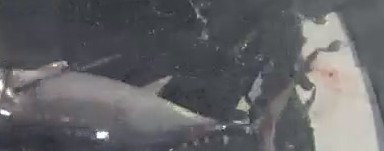
\includegraphics[width=.9\linewidth]{img/Quality/albLabelpoor07917_2019-06-22_12-57-43.jpg}
\end{center}

This is more evident from the original image:

\begin{center}
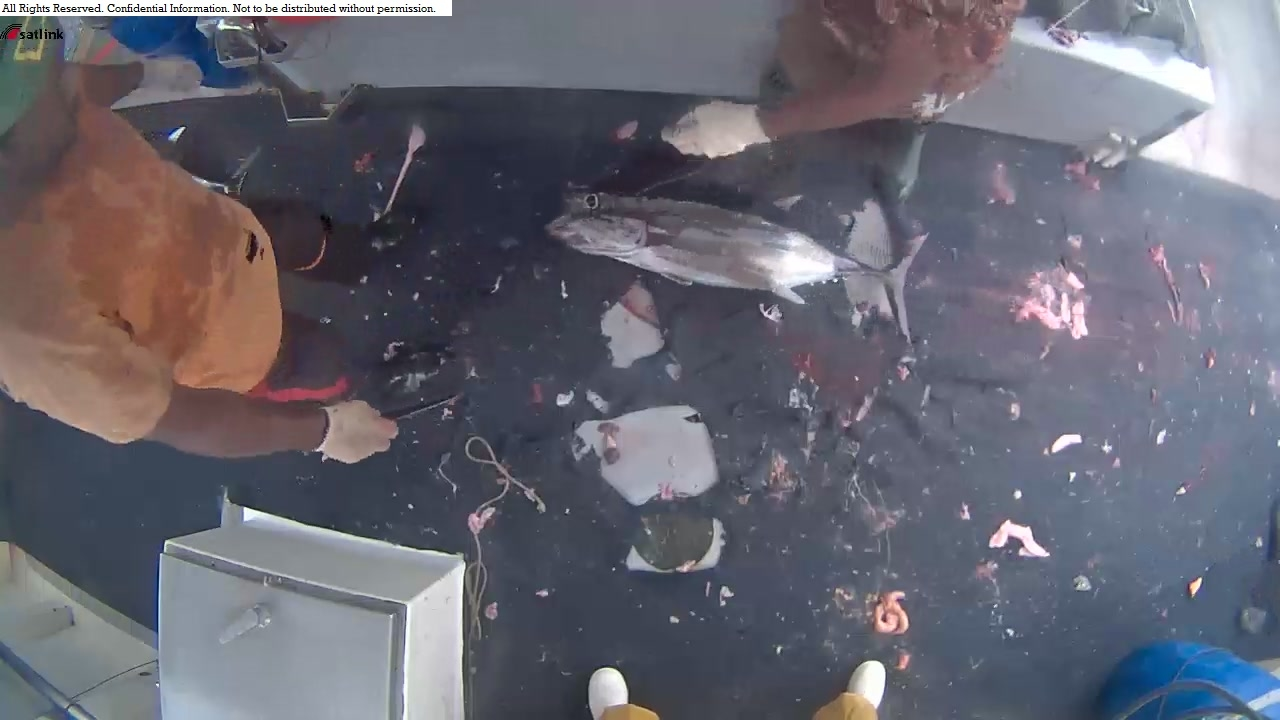
\includegraphics[width=.9\linewidth]{img/Quality/albLabel07917orig_2019-06-22_12-57-57.jpg}
\end{center}

\subsubsection{No Fish}
\label{sec:org3f4e828}
Naturally the original image has no fish:

\begin{center}
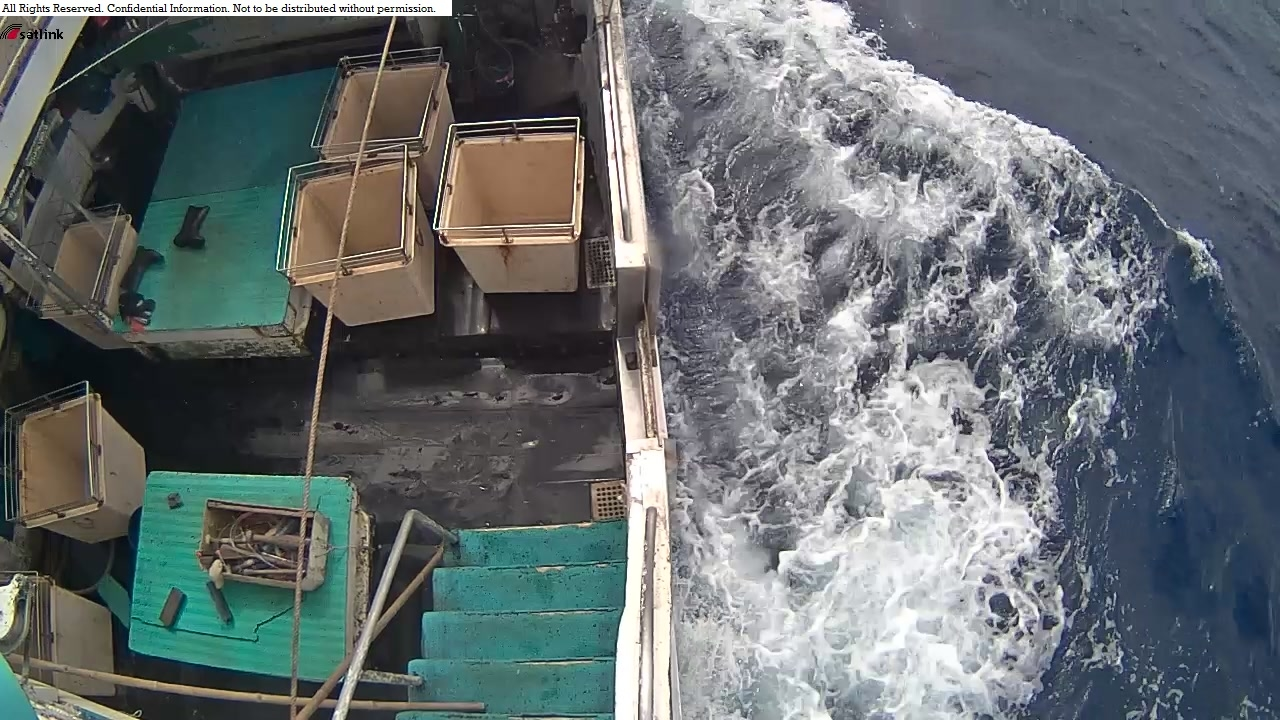
\includegraphics[width=.9\linewidth]{img/Quality/nofish_00008-labelOrig_2019-06-22_12-58-24.jpg}
\end{center}

Equally unsurprisingly, the no-fish bounding box is, \textbf{not fish}:

\begin{center}

\includegraphics[width=.9\linewidth]{img/Quality/nofish_00008-label_2019-06-22_12-58-47.jpg}
\end{center}

\rg{This is great news! We can totally ignore the no-fish bounding box!}
\subsection{Preprocessing}
\label{sec:org1b5eace}

\begin{itemize}
\item Visual inspection of the images showed that a lot of them (but not all) had a
water-mark.
\end{itemize}


\begin{center}
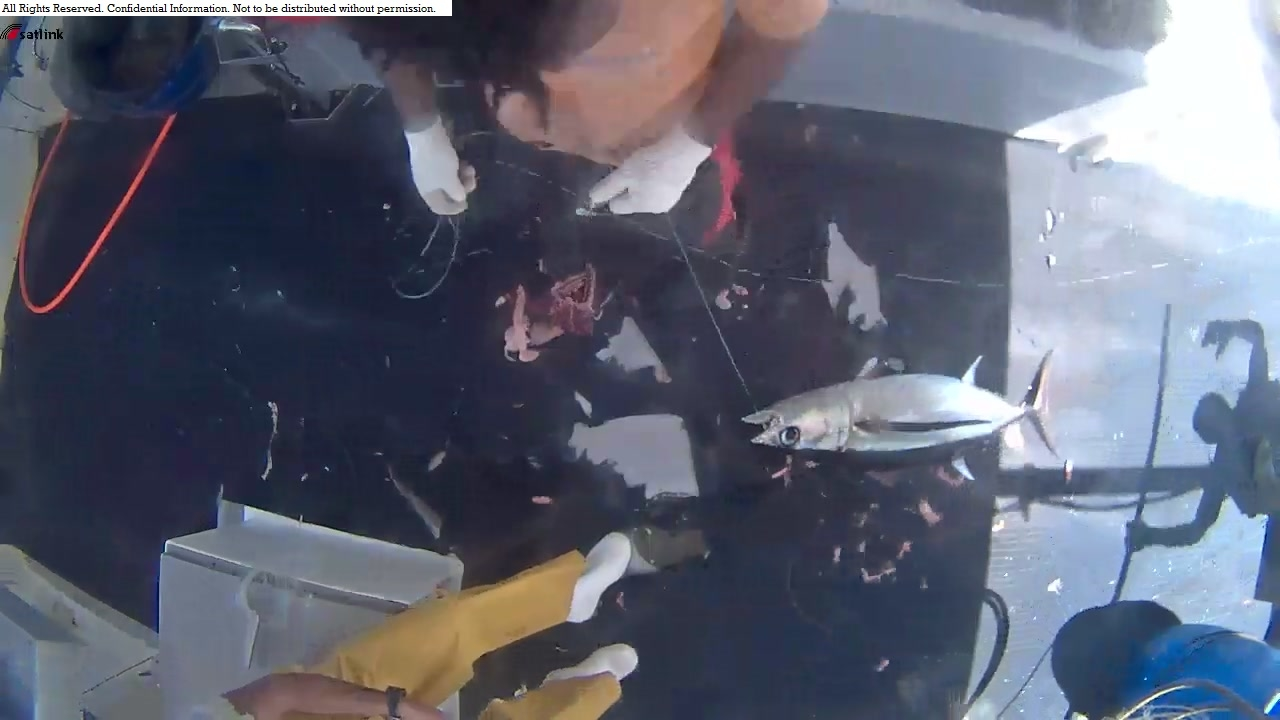
\includegraphics[width=.9\linewidth]{img/Data_Preprocessing/img_00299_2019-06-22_12-06-01.jpg}
\end{center}
\end{document}
